\documentclass[12pt]{article}
\usepackage[margin=1in]{geometry}
\usepackage{amsmath,amssymb,amsthm,booktabs,array}
\usepackage{microtype}
\usepackage{newcomputermodern}
\usepackage[most]{tcolorbox}
\usepackage{tikz}
\usetikzlibrary{arrows.meta,positioning}
\usepackage[hidelinks]{hyperref}
\usepackage{enumitem,needspace}
\setcounter{tocdepth}{1}
\AddToHook{cmd/section/before}{\Needspace{7\baselineskip}}
\AddToHook{cmd/subsection/before}{\Needspace{5\baselineskip}}
\setlist{itemsep=2pt,topsep=4pt}
\newtcolorbox{remarkbox}[1][Note]{colback=gray!5,colframe=gray!60,title={#1},fonttitle=\bfseries,arc=2mm,boxrule=.6pt,breakable}
\newtcolorbox{correction}[1][Correction]{colback=red!3,colframe=red!55!black,title={#1},fonttitle=\bfseries,arc=2mm,boxrule=.6pt,breakable}
\newtcolorbox{todo}[1][TODO from the manuscript]{colback=yellow!8,colframe=orange!70!black,title={#1},fonttitle=\bfseries,arc=2mm,boxrule=.6pt,breakable}
\newtcolorbox{supplement}[1][Lecture supplement]{colback=blue!3,colframe=blue!50!black,title={#1},fonttitle=\bfseries,arc=2mm,boxrule=.6pt,breakable}
\newcommand{\E}{\mathbb E}
\newcommand{\Prob}{\mathbb P}
\newcommand{\Var}{\operatorname{Var}}
\newcommand{\Cov}{\operatorname{Cov}}
\newcommand{\pa}{\operatorname{Pa}}
\newcommand{\de}{\operatorname{De}}
\newcommand{\an}{\operatorname{An}}
\newcommand{\nd}{\operatorname{Nd}}
\newcommand{\doo}{\operatorname{do}}
\newcommand{\ind}{\mathrel{\perp\!\!\!\perp}}
\newcommand{\nind}{\mathrel{\not\!\perp\!\!\!\perp}}
\newcommand{\dsep}{\mathrel{\perp\!\!\!\perp}_{d}}
\newcommand{\source}[1]{\par\smallskip{\small\color{gray!80!black}\textit{Manuscript: #1.}}\par}
\setlength{\parindent}{0pt}
\setlength{\parskip}{6pt}
\setlength{\emergencystretch}{2em}
\tikzset{v/.style={circle,draw=blue!45!black,fill=blue!3,minimum size=8mm,inner sep=2pt},edge/.style={-{Stealth[length=2mm]},thick}}
\author{Liang-Cheng Chen}
\date{Spring 2026\quad /\quad Typeset October 25, 2026}
% TASK.md explicitly requests double-dollar delimiters for INLINE math.
% Make the dollar character active so paired $$...$$ means ensuremath,
% not TeX display math. Display formulas use equation/align exclusively.
\catcode`\$=\active
\protected\long\def$$#1$${\ensuremath{#1}}

\title{STAT 566: Causal Modeling\\[.4em]\large Edited Course Notes}
\begin{document}
\maketitle
\begin{remarkbox}[About this edition]
Transcribed from four handwritten PDFs (53 pages), translated into English, and checked against the course lectures. Original numbering is retained: Notes 1, 2, 3, and 5. Yellow boxes preserve TODOs; red boxes document corrections; blue boxes mark supplements. No Note 4 was supplied. See \texttt{SOURCE-MAP.md} for the page-by-page coverage map and \texttt{LOG.log} for limitations.
\end{remarkbox}
\tableofcontents
\clearpage
\part{Note 01: Potential Outcomes, Randomized Experiments, and Partial Identification}
\section{Potential outcomes and causal estimands}
\source{stat566-note01, pp. 1--2 (April 2)}
Let $$A\in\{0,1\}$$ denote treatment and $$Y(a)$$ the potential outcome under treatment $$a$$. The observed outcome is $$Y=Y(A)$$ under consistency. Define
\begin{align}
\tau=\operatorname{ATE}&=\E[Y(1)-Y(0)],\\
\operatorname{ATT}&=\E[Y(1)-Y(0)\mid A=1],\\
\operatorname{ATC}&=\E[Y(1)-Y(0)\mid A=0].
\end{align}
Writing $$p=\Prob(A=1)$$, the law of total expectation gives
\begin{equation}
\operatorname{ATE}=p\operatorname{ATT}+(1-p)\operatorname{ATC}.
\end{equation}
These are population targets, not estimators. Their numerical values need not agree in an observational study.

For a binary outcome, classify units by their pair of potential outcomes:
\begin{center}
\begin{tabular}{lccc}\toprule
Outcome response type & $$Y(0)$$ & $$Y(1)$$ & Effect\\\midrule
Always has outcome & 1&1&0\\
Never has outcome & 0&0&0\\
Helped / responder & 0&1&1\\
Harmed & 1&0&$$-1$$\\\bottomrule
\end{tabular}
\end{center}
Thus
\begin{align}
\E[Y(1)]&=\Prob(\text{always})+\Prob(\text{helped}),\\
\E[Y(0)]&=\Prob(\text{always})+\Prob(\text{harmed}),\\
\tau&=\Prob(\text{helped})-\Prob(\text{harmed}),\\
\operatorname{ATT}&=\Prob(\text{helped}\mid A=1)-\Prob(\text{harmed}\mid A=1).
\end{align}
\begin{correction}[Response types versus compliance types]
The manuscript calls the first two rows ``always-taker'' and ``never-taker.'' Here the table concerns outcomes, so ``always has outcome'' and ``never has outcome'' are more precise. IV compliance types instead concern potential \emph{treatment uptake}, $$A(0),A(1)$$; see Note 5.
\end{correction}
\begin{remarkbox}[Question in the margin: what if the harmed proportion is known?]
The identity for $$\tau$$ is valid irrespective of whether either response proportion is known. Knowing the harmed proportion alone does not identify the helped proportion. If randomization identifies $$\tau$$ and the harmed proportion is supplied separately, then their sum identifies the helped proportion. Even an RCT generally identifies only the marginal distributions of $$Y(0)$$ and $$Y(1)$$, not their joint distribution.
\end{remarkbox}

\section{SUTVA, consistency, and randomization}
\source{stat566-note01, pp. 2--4}
SUTVA (stable unit treatment value assumption) packages no interference and the absence of relevant hidden treatment versions. The course also spells out consistency separately.
\begin{enumerate}
\item \textbf{Treatment variation irrelevance.} If versions $$k$$ and $$k'$$ represent the same treatment level $$a$$, then $$Y_i(a,k)=Y_i(a,k')$$. Different doses should not be silently treated as equivalent versions if they change the outcome.
\item \textbf{Consistency.} If $$A_i=a$$, then $$Y_i=Y_i(a)$$. Equivalently,
\begin{equation}
Y_i=A_iY_i(1)+(1-A_i)Y_i(0).
\end{equation}
\item \textbf{No interference.} A unit's potential outcome depends on its own treatment, not the treatment assignments to other units:
\begin{equation}
Y_i(a_1,\ldots,a_n)=Y_i(a_i).
\end{equation}
Vaccination is a counterexample when other people's vaccination protects an untreated person.
\end{enumerate}
\begin{todo}[TODO / questions, p. 3: consistency and ``EQC?'']
The original asks to reread the reference and contains the shorthand ``EQC?'' twice; that abbreviation cannot be reliably expanded. The relevant equality is
\begin{equation}
\E[Y(1)\mid A=1]=\E[Y\mid A=1],
\end{equation}
which follows from consistency alone. In contrast, replacing $$\E[Y(1)\mid A=1]$$ by $$\E[Y(1)]$$ needs exchangeability. The ambiguous abbreviation is preserved here rather than guessed.
\end{todo}

In a randomized experiment, treatment assignment is independent of potential outcomes (and baseline covariates under simple randomization):
\begin{equation}
A\ind (Y(0),Y(1),Z).
\end{equation}
Consequently, for $$a=0,1$$ with positive assignment probability,
\begin{align}
\E[Y(a)]&=\E[Y(a)\mid A=a]=\E[Y\mid A=a],\\
\tau&=\E[Y\mid A=1]-\E[Y\mid A=0].
\end{align}
Population ATE, ATT, and ATC then agree. A realized randomized sample need not have exact balance: baseline summary statistics diagnose chance imbalance but do not prove or disprove the assignment mechanism.
\begin{correction}[Consistency is not independence from intention]
Consistency is the equality $$Y=Y(A)$$, not an independence statement about a person's intention to receive treatment. Random assignment of an offer identifies an intention-to-treat effect; noncompliance creates a separate question about actual treatment receipt.
\end{correction}

\section{Neyman estimation and Fisher randomization inference}
\source{stat566-note01, pp. 4--5; Lecture 1, randomization inference}
For a completely randomized assignment of $$n_1$$ treated and $$n_0=n-n_1$$ controls, the difference in sample means estimates the finite-population ATE:
\begin{align}
\widehat\tau&=\overline Y_1-\overline Y_0
=\frac1{n_1}\sum_{i:A_i=1}Y_i-\frac1{n_0}\sum_{i:A_i=0}Y_i,\\
\tau_n&=\frac1n\sum_{i=1}^n\{Y_i(1)-Y_i(0)\},\qquad
\E_A[\widehat\tau]=\tau_n.
\end{align}
Here the potential outcomes are fixed; randomness is over the treatment assignments. Define finite-population variances using all $$n$$ units:
\begin{align}
S_a^2&=\frac1{n-1}\sum_{i=1}^n\{Y_i(a)-\overline Y(a)\}^2,\\
S_\tau^2&=\frac1{n-1}\sum_{i=1}^n\{Y_i(1)-Y_i(0)-\tau_n\}^2.
\end{align}
Then
\begin{equation}
\Var_A(\widehat\tau)=\frac{S_1^2}{n_1}+\frac{S_0^2}{n_0}-\frac{S_\tau^2}{n}.
\end{equation}
The within-arm sample variances $$s_a^2$$ give the usual conservative estimator
\begin{equation}
\widehat V=\frac{s_1^2}{n_1}+\frac{s_0^2}{n_0},\qquad
\E_A[\widehat V]=\Var_A(\widehat\tau)+\frac{S_\tau^2}{n}.
\end{equation}
\begin{correction}[Variance notation and the asymptotic pivot]
The manuscript mixes sample variances computed within the observed arms with the finite-population variances in Neyman's exact formula. Moreover, $$\widehat V\geq\Var_A(\widehat\tau)$$ is not guaranteed for every realized sample; conservativeness is in expectation. A central limit theorem concerns the centered statistic $$(\widehat\tau-\tau_n)/\sqrt{\Var_A(\widehat\tau)}$$. Using $$\widehat V$$ typically gives conservative large-sample confidence intervals under suitable regularity conditions, rather than an automatically exact standard normal pivot.
\end{correction}

Fisher's sharp null is
\begin{equation}
H_0^{\mathrm{sharp}}:\quad Y_i(1)=Y_i(0)\quad\text{for every }i.
\end{equation}
It implies $$\tau_n=0$$, but the converse fails: positive and negative individual effects can average to zero.
\begin{todo}[TODO, p. 5: reread Fisher's exact test / fill notes up to 10:08]
Under the sharp null every missing potential outcome is imputed by the observed outcome. Choose a statistic such as $$T=\overline Y_1-\overline Y_0$$, enumerate assignments allowed by the original design, recompute $$T$$ for each, and calculate the fraction at least as extreme as the observed statistic:
\begin{equation}
p_{\mathrm{exact}}=\frac{1}{|\mathcal A|}\sum_{a\in\mathcal A}
\mathbf1\{|T(a,Y)|\geq|T(A^{\mathrm{obs}},Y)|\}.
\end{equation}
This expression assumes equally likely assignments. Use design probabilities otherwise. Monte Carlo sampling of assignments approximates enumeration. The timestamp identifies a missing recording segment; its exact contents are unavailable, so this box supplies the lecture's core method rather than reconstructing an unheard segment.
\end{todo}

\section{Partial identification and Manski bounds}
\source{stat566-note01, pp. 6--7 (April 7); Lecture 2, Sections 1--2}
Identification asks what is determined by the population observed-data law; estimation approximates that quantity from a sample. Without exchangeability, the ATE need not be point identified. Assume both potential outcomes lie in a known interval $$[L,U]$$, and write $$\mu_a=\E[Y\mid A=a]$$, $$p=\Prob(A=1)\in(0,1)$$, and $$q=1-p$$. Consistency gives
\begin{align}
\E[Y(1)]&=p\mu_1+q\E[Y(1)\mid A=0],\\
\E[Y(0)]&=q\mu_0+p\E[Y(0)\mid A=1].
\end{align}
The missing counterfactual means can range over $$[L,U]$$, so
\begin{align}
p\mu_1+qL&\leq\E[Y(1)]\leq p\mu_1+qU,\\
q\mu_0+pL&\leq\E[Y(0)]\leq q\mu_0+pU.
\end{align}
Subtract opposite endpoints to obtain sharp bounds:
\begin{align}
\tau_L&=p(\mu_1-U)+q(L-\mu_0),\\
\tau_U&=p(\mu_1-L)+q(U-\mu_0),\\
\tau&\in[\tau_L,\tau_U],\qquad \tau_U-\tau_L=U-L.
\end{align}
Sharp means every endpoint is attainable by some potential-outcome distribution consistent with the observed law and maintained assumptions. Bounded support alone gives $$[L-U,U-L]$$, of width $$2(U-L)$$; observing treatment and outcome cuts that width in half.
\begin{remarkbox}[Questions, p. 7: can the lower endpoint be zero?]
Yes, $$L=0$$ is allowed; use whatever support is substantively justified. For binary outcomes $$[L,U]=[0,1]$$, the trivial ATE range is $$[-1,1]$$, but Manski's data-dependent interval has width 1. For $$p=.4$$, $$\mu_1=.7$$, $$\mu_0=.5$$, the interval is $$[-.42,.58]$$. The naive contrast .2 does not identify the ATE. A bounded \emph{observed} outcome alone does not establish bounds on unobserved potential outcomes without the corresponding maintained support restriction.
\end{remarkbox}

\section{Monotone treatment response and selection}
\source{stat566-note01, pp. 8--9; Lecture 2, Section 3}
\textbf{MTR} (monotone treatment response) assumes $$Y_i(1)\geq Y_i(0)$$ for every unit. If larger values are beneficial, it rules out harm. This is a substantive restriction, not a general property of treatments. It implies
\begin{align}
\E[Y(1)\mid A=0]&\geq\mu_0,\\
\E[Y(0)\mid A=1]&\leq\mu_1,\\
\tau&\in[0,\tau_U].
\end{align}
\begin{todo}[TODO, p. 8: complete the MTR bound]
The upper endpoint remains $$p(\mu_1-L)+q(U-\mu_0)$$; it is generally not simply $$U$$. A zero effect for every unit achieves the lower endpoint while respecting each observed outcome. Setting untreated units' missing treated outcomes to $$U$$ and treated units' missing control outcomes to $$L$$ achieves the upper endpoint and respects MTR.
\end{todo}
\textbf{Positive MTS} (monotone treatment selection) assumes
\begin{equation}
\E[Y(t)\mid A=1]\geq\E[Y(t)\mid A=0],\qquad t=0,1.
\end{equation}
It describes positive sorting into treatment on potential outcomes, not nonnegative treatment effects. Thus
\begin{align}
\E[Y(1)\mid A=0]&\leq\mu_1, & \E[Y(0)\mid A=1]&\geq\mu_0,\\
\tau&\in[\tau_L,\mu_1-\mu_0] &&\text{under MTS alone},\\
\tau&\in[0,\mu_1-\mu_0] &&\text{under MTR and MTS}.
\end{align}
\begin{correction}[The lower bound zero needs MTR]
The manuscript's final interval implicitly combines MTR and MTS. Positive MTS alone does not prevent negative causal effects. If $$\mu_1<\mu_0$$, the combined assumptions are incompatible with the observed law. Some settings motivate negative rather than positive selection; the direction must be justified. These are identification bounds, not confidence intervals for estimated endpoints.
\end{correction}
\section*{Lecture cross-reference}
Ema Perkovi\'c, STAT 566, Spring 2026: Lecture 1, \emph{Introduction and Randomized Experiments} (SUTVA, Neyman estimation, Fisher inference); Lecture 2, \emph{Manski Bounds and Partial Identification}, Sections 1--3. Local source filenames and full manuscript coverage are listed in \texttt{SOURCE-MAP.md}.

\clearpage
\part{Note 02: Graphical Models, Markov Properties, and Causal Identification}
\section{Graphs, paths, and Bayesian networks}
\source{stat566-note02, pp. 1--4 (April 9); Lecture 3, Sections 1--2}
A graph $$G=(V,E)$$ has nodes $$V=\{V_1,\ldots,V_k\}$$ and edges $$E$$. In a directed acyclic graph (DAG), every edge has a direction and no directed cycle is allowed. This encodes the absence of instantaneous feedback; feedback over time can sometimes be represented by distinct time-indexed nodes.

A path is a sequence of \emph{distinct} nodes with adjacent consecutive nodes, irrespective of arrow direction. A directed path follows arrows throughout. For the running example, take
\begin{equation}
Z\to A,\quad Z\to Y,\quad A\to M,\quad M\to Y.
\end{equation}
\begin{center}
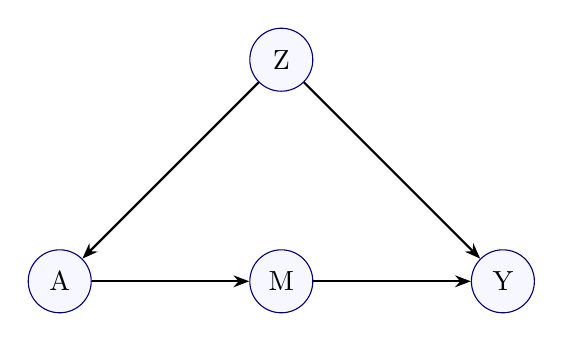
\begin{tikzpicture}[node distance=20mm]
\node[v] (a) {A};\node[v,right=of a] (m) {M};\node[v,right=of m] (y) {Y};\node[v,above=of m] (z) {Z};
\draw[edge] (z)--(a);\draw[edge] (z)--(y);\draw[edge] (a)--(m);\draw[edge] (m)--(y);
\end{tikzpicture}
\end{center}
Here $$A,M,Y,Z$$ is a path (the final edge is traversed backward), but $$M,Z,Y$$ is not a path because $$M,Z$$ are not adjacent. The sequence $$A,M,Y,Z,A$$ repeats $$A$$ and is not a path under this convention. Relative to treatment $$A$$ and outcome $$Y$$, $$M$$ is a mediator and $$Z$$ is a common cause.
\begin{description}
\item[Parents / children:] $$\pa(V_j)$$ are nodes with an edge into $$V_j$$; children have an edge from $$V_j$$.
\item[Ancestors / descendants:] $$\an(V_j)$$ can reach $$V_j$$ by directed paths; $$\de(V_j)$$ are reachable from $$V_j$$. We include the node itself in these sets, matching the handwritten convention. Define $$\nd(V_j)=V\setminus\de(V_j)$$.
\item[Root / sink:] A root has no parents; a sink has no children. Every finite nonempty DAG has at least one root and at least one sink, potentially several.
\end{description}
For this example, $$\an(Y)=\{Z,A,M,Y\}$$ and $$\de(Y)=\{Y\}$$. A topological ordering lists parents before children; $$Z,A,M,Y$$ is one such ordering.

A Bayesian network pairs a DAG with a distribution that factorizes according to it. This supplies probabilistic semantics. A causal model adds assumptions about autonomous mechanisms and how interventions modify them; a Bayesian network alone does not license a do-operator interpretation.

\section{Factorization, the LMP, and the GMP}
\source{stat566-note02, pp. 3, 7--8; Lecture 3, Sections 2.2 and 4.3}
\subsection{Three forms of the Markov property}
Let $$p$$ denote a joint probability mass function or density. Its \textbf{Markov factorization} is
\begin{equation}\label{eq:factor}
p(v_1,\ldots,v_k)=\prod_{j=1}^k p(v_j\mid\pa(v_j)).
\end{equation}
The \textbf{local Markov property} (LMP) is, for every node,
\begin{equation}\label{eq:lmp}
V_j\ind \nd(V_j)\setminus\pa(V_j)\mid\pa(V_j).
\end{equation}
Explicitly removing parents from the non-descendant set keeps the three sets disjoint. The shorthand ``independent of non-descendants given parents'' expresses the same idea.

The \textbf{global Markov property} (GMP) states that for every three disjoint sets of nodes $$B,C,S$$,
\begin{equation}\label{eq:gmp}
B\dsep C\mid S\text{ in }G\quad\Longrightarrow\quad B\ind C\mid S\text{ under }P.
\end{equation}
The left side is a property of the graph. The right side is a property of a probability distribution.
\begin{supplement}[LMP, GMP, and factorization are equivalent]
For a DAG and an ordinary finite discrete distribution or a joint law with suitable conditional densities,
\begin{equation}
\boxed{\text{LMP}\quad\Longleftrightarrow\quad\text{factorization}\quad\Longleftrightarrow\quad\text{GMP}.}
\end{equation}
These are equivalent descriptions of the Markov model, not three unrelated assumptions. Lecture 3 states the result for strictly positive distributions, which is a convenient sufficient setting. For DAGs strict positivity is not essential: conditionals are interpreted on their support (or as probability kernels almost surely). Positivity for causal adjustment is a different requirement concerning treatment overlap.
\end{supplement}
\subsection{Why LMP gives factorization}
Choose a topological order $$V_1,\ldots,V_k$$ and write $$\operatorname{Pre}_j=\{V_1,\ldots,V_{j-1}\}$$. No predecessor is a descendant of $$V_j$$, and all parents occur among predecessors. The ordinary probability chain rule always gives
\begin{equation}
p(v_1,\ldots,v_k)=\prod_{j=1}^k p(v_j\mid v_1,\ldots,v_{j-1}).
\end{equation}
LMP and decomposition of conditional independence imply
\begin{equation}
V_j\ind\operatorname{Pre}_j\setminus\pa(V_j)\mid\pa(V_j),
\end{equation}
so each full-history conditional reduces to the parent-only conditional. This yields equation~\eqref{eq:factor}. Conversely, factorization implies the graphical separation statements in GMP; in particular, a node's parents d-separate it from its other non-descendants, yielding LMP.
\begin{supplement}[Why factorization gives GMP: proof outline]
To assess $$B\dsep C\mid S$$, retain the ancestors of $$B\cup C\cup S$$. Marginalizing all other nodes in reverse topological order removes their normalized conditional factors. Moralize the remaining DAG: connect co-parents and erase arrowheads. Each remaining factor involves a node and its parents, a clique in this moral graph. The d-separation criterion is equivalent to ordinary separation by $$S$$ in this ancestral moral graph. After fixing $$S=s$$, factors can therefore be grouped into products over components on the two sides, and normalization yields $$p(b,c\mid s)=p(b\mid s)p(c\mid s)$$. This is the distributional statement in GMP. Moralizing the \emph{whole} graph without first restricting to the relevant ancestors can give the wrong answer.
\end{supplement}

\subsection{Worked factorization and a correction}
For the four-node example, the chain rule and Markov restrictions give
\begin{align}
p(z,a,m,y)&=p(z)p(a\mid z)p(m\mid a,z)p(y\mid z,a,m)\\
&=p(z)p(a\mid z)p(m\mid a)p(y\mid z,m).
\end{align}
The reductions use
\begin{equation}
M\ind Z\mid A,\qquad Y\ind A\mid (Z,M).
\end{equation}
\begin{correction}[The missing conditioning variable, manuscript p. 3]
The handwritten statement $$A\ind Y\mid M$$ is generally false because $$A\leftarrow Z\to Y$$ remains open. The correct parent-based statement is $$Y\ind A\mid Z,M$$. Blocking the mediated path alone does not block confounding.
\end{correction}
Adding $$Z\to M$$ allows a larger Markov model. A distribution satisfying the original factorization still satisfies the enlarged graph's factorization by letting $$p(m\mid a,z)=p(m\mid a)$$. The enlarged graph does not require that equality. It also does not make that same distribution faithful to the enlarged graph.
\begin{remarkbox}[A practical way to use the three formulations]
Use factorization to write or simulate a distribution. Use LMP to derive parent-based conditional independencies and simplify the chain rule. Use GMP to answer a specific independence query between arbitrary sets. None of these directions says that every d-connected pair must be dependent; that further conclusion needs faithfulness.
\end{remarkbox}

\section{d-separation and the three path motifs}
\source{stat566-note02, pp. 5--8 (April 14); Lecture 3, Section 3}
A collider is an \emph{interior node on a particular path} where the two adjacent path edges both point inward. Collider status is path-relative. For disjoint conditioning set $$S$$, a path is open (d-connecting) if every non-collider on it is outside $$S$$ and every collider is in $$\an(S)$$. Equivalently, each collider has itself or a descendant in $$S$$. Otherwise the path is blocked. Two sets are d-separated if \emph{every} path between them is blocked.
\begin{center}
\begin{tabular}{lll}\toprule
Motif & Without conditioning & Given middle node\\\midrule
Chain: $$X\to M\to Y$$ & Open & Blocked\\
Fork: $$X\leftarrow C\to Y$$ & Open & Blocked\\
Collider: $$X\to C\leftarrow Y$$ & Blocked & Open\\\bottomrule
\end{tabular}
\end{center}
The reverse chain $$X\leftarrow M\leftarrow Y$$ behaves like the first row. Conditioning on a descendant of a collider also activates the collider.
\begin{correction}[Fork and collider were interchanged on p. 5]
A fork has arrows \emph{out of} the middle node; a collider has arrows \emph{into} it. The handwritten motif labels conflict with their arrows. The table corrects the labels and gives the corresponding open/blocked behavior.
\end{correction}
\begin{supplement}[Conditioning is not monotone in d-separation]
Adding a variable to $$S$$ may block a non-collider path or activate a collider path. Thus a superset of a valid adjustment set need not be valid. To check a query: enumerate paths, identify colliders separately on each path, apply both blocking rules, and verify that no open path remains. An adjacent pair cannot be d-separated by any set excluding the endpoints, because their one-edge path has no interior node to block.
\end{supplement}
\subsection{Berkson's paradox and descendant conditioning}
The graph $$D_1\to H\leftarrow D_2$$ represents two diseases causing hospitalization. Under the graph's Markov model $$D_1\ind D_2$$, but restricting attention to hospitalized patients conditions on $$H$$ and can induce association. If $$H\to B$$, selecting on a hospital bill $$B$$ can do the same. The direction and strength of induced association depend on the mechanisms; the graph alone does not determine its sign.

For $$Z\to A\leftarrow U$$, $$A\to M\to Y$$, $$Z\to Y$$, $$U\to W$$, examine:
\begin{align}
Z&\dsep U &&\text{without conditioning},\\
A&\dsep W\mid U &&\text{the fork through }U\text{ is blocked}.
\end{align}
Conditioning on $$A$$, on $$M$$, or on $$Y$$ activates the collider at $$A$$ because $$M,Y$$ are descendants of $$A$$. Hence $$Z$$ and $$U$$ are then d-connected. These are graphical statements; dependence follows under faithfulness.

\section{Faithfulness and Markov equivalence}
\source{stat566-note02, pp. 7--8, 18; Lecture 3, Section 4}
The Markov assumption gives graphical separation $$\Rightarrow$$ statistical independence. Faithfulness gives the converse:
\begin{equation}
B\ind C\mid S\text{ under }P\quad\Longrightarrow\quad B\dsep C\mid S\text{ in }G.
\end{equation}
Together they make the two independence structures coincide. Faithfulness rules out accidental independencies caused by exact parameter cancellation.
\begin{supplement}[An explicit cancellation example]
Let independent Gaussian errors generate
\begin{equation}
A\leftarrow\epsilon_A,\quad M\leftarrow A+\epsilon_M,\quad
Y\leftarrow M-A+\epsilon_Y.
\end{equation}
The DAG has $$A\to M\to Y$$ and $$A\to Y$$. Substitution gives $$Y=\epsilon_M+\epsilon_Y$$, so $$A\ind Y$$ despite d-connection. The model is Markov but unfaithful. Independent errors alone do not guarantee faithfulness.
\end{supplement}
Two DAGs are \textbf{Markov equivalent} if they have the same d-separation statements. The graphical characterization is: same skeleton (undirected adjacencies) and same unshielded colliders (v-structures).
\begin{align}
V_1\to V_2\to V_3,\quad V_1\leftarrow V_2\to V_3,\quad
V_1\leftarrow V_2\leftarrow V_3
\end{align}
form one equivalence class and imply $$V_1\ind V_3\mid V_2$$. The graph $$V_1\to V_2\leftarrow V_3$$ is a different class and implies marginal independence of its endpoints.
\begin{correction}[Causality, faithfulness, and identification]
A causal DAG need not be faithful to its distribution. Faithfulness is especially useful for causal discovery from conditional independencies, but back-door identification for a \emph{given} correct causal DAG does not require faithfulness. Observational data generally identify only an equivalence class. Sufficiently rich intervention data can orient more edges under additional assumptions; ``all interventions imply a unique DAG'' is not unconditional, since redundant edges and unfaithful mechanisms can hide causal distinctions.
\end{correction}

\section{Structural causal models and randomization}
\source{stat566-note02, pp. 4, 9--11, 21; Lectures 3 and 3b}
An acyclic structural causal model specifies assignments
\begin{equation}
V_j\leftarrow f_j(\pa(V_j),\epsilon_j),\qquad j=1,\ldots,k,
\end{equation}
with mutually independent exogenous errors for the causally sufficient DAG model. A topological order makes recursive generation possible. Pairwise independence of errors is generally insufficient; mutual independence is intended. Gaussianity and linearity are optional modeling choices.
\begin{align}
Z&\leftarrow\epsilon_Z, & W&\leftarrow\epsilon_W,\\
A&\leftarrow\mathbf1\{\alpha_{ZA}Z+\alpha_{WA}W+\epsilon_A>0\},\\
Y&\leftarrow\beta A+\gamma Z+\epsilon_Y.
\end{align}
This threshold model illustrates a binary treatment. Arbitrary nonlinear functions can replace the linear expressions. Additive noise $$f(\pa(V_j))+\epsilon_j$$ is more restrictive than a general function $$f(\pa(V_j),\epsilon_j)$$.
\begin{todo}[TODO, p. 21: add notes about SCMs]
To obtain $$Y(a)$$, retain the same exogenous errors and replace only the assignment for $$A$$ by $$A\leftarrow a$$; then recursively recompute its descendants. If a unit naturally has $$A=a$$, the recomputed outcome equals its observed outcome (consistency). The functions encode relevant treatment versions and, in a per-unit model with no cross-unit arguments, no interference. Shared latent causes can be represented explicitly by extra nodes; dependent errors generally invalidate the simple observed-variable DAG factorization.
\end{todo}
A randomized treatment replaces the assignment for $$A$$ by an independent random draw, for example $$A\leftarrow\epsilon_A^{\mathrm{RCT}}\sim\operatorname{Bernoulli}(.5)$$. Incoming edges to $$A$$ disappear, but its outgoing causal mechanisms remain.

\subsection{Parametric inference and adjustment in an RCT}
For two independent normal samples with a common variance, the pooled two-sample statistic is
\begin{align}
s_p^2&=\frac{(n_1-1)s_1^2+(n_0-1)s_0^2}{n_1+n_0-2},\\
t&=\frac{\overline Y_1-\overline Y_0-\tau_0}{s_p\sqrt{1/n_1+1/n_0}}.
\end{align}
Under the null it has a $$t_{n_1+n_0-2}$$ distribution in this parametric setting. Under a nonzero alternative, the noncentrality parameter is $$(\tau-\tau_0)/(\sigma\sqrt{1/n_1+1/n_0})$$. Power is $$1-\beta_{\mathrm{II}}=\Prob(\text{reject }H_0\mid\text{specified alternative})$$.
\begin{correction}[The standard error needs the arm-size factors]
The handwritten denominator only displays a pooled variance. The statistic requires $$s_p\sqrt{1/n_1+1/n_0}$$. This parametric result is distinct from finite-population randomization inference. Use Welch's test or robust inference when the equal-variance model is inappropriate.
\end{correction}
In an RCT, conditioning on a mediator $$A\to M\to Y$$ blocks part of the total effect. Conditioning on a common effect $$A\to C\leftarrow Y$$ can introduce selection bias. Baseline prognostic covariates may improve precision, but precision gains are not automatic and inference must match the adjustment method. The graph and the estimator jointly determine the interpretation.

\section{Interventions and truncated factorization}
\source{stat566-note02, pp. 12--13, 18--19 (April 21--23); Lecture 4, Section 1}
For a causal DAG with invariant mechanisms, $$\doo(A=a)$$ replaces the treatment mechanism by a constant. Let $$G_{\overline A}$$ denote removal of incoming edges to $$A$$. The post-intervention law on the other variables is
\begin{equation}
p(v_{-A}\mid\doo(A=a))=
\left.\prod_{V_j\neq A}p(v_j\mid\pa(v_j))\right|_{A=a}.
\end{equation}
If the joint law includes $$A$$, multiply this product by a point mass at $$a$$ (an indicator for a discrete treatment, a Dirac measure for a continuous one).

For $$Z\to A\to Y$$ and $$Z\to Y$$,
\begin{align}
p(z,a,y)&=p(z)p(a\mid z)p(y\mid a,z),\\
p(z,y\mid\doo(A=a))&=p(z)p(y\mid a,z),\\
p(y\mid\doo(A=a))&=\int p(y\mid a,z)\,dP(z),\\
\E[Y(a)]&=\int\E[Y\mid A=a,Z=z]\,dP(z).
\end{align}
In contrast, ordinary conditioning averages over $$P(Z\mid A=a)$$, which generally differs from $$P(Z)$$. Two observationally equivalent factorizations can imply different intervention laws because they assign different causal mechanisms.
\begin{correction}[Avoid a stray treatment indicator]
Once $$A=a$$ is fixed and $$A$$ is not part of the random vector, $$p(y\mid\doo(A=a))$$ does not contain an additional $$\mathbf1\{A=a\}$$. The indicator belongs only in a joint post-intervention law that still includes the treatment variable.
\end{correction}

\section{Back-door adjustment and choosing a set}
\source{stat566-note02, pp. 13--20; Lecture 4, Sections 2--4}
An observed set $$S$$ is an adjustment set if
\begin{equation}
p(y\mid\doo(A=a))=\int p(y\mid A=a,S=s)\,dP(s).
\end{equation}
For discrete variables, replace the integral by a sum. Pearl's back-door criterion is a sufficient graphical condition:
\begin{enumerate}
\item $$S$$ contains no descendants of $$A$$ and excludes $$A,Y$$.
\item $$S$$ blocks every path from $$A$$ to $$Y$$ whose first edge points into $$A$$.
\end{enumerate}
If no directed path leads from A to Y, intervening on A cannot change Y in the stated acyclic SCM. A single reverse arrow is not by itself enough to conclude this in a larger graph; check for other directed paths.

A back-door path need not be directed toward $$A$$ along its entire length. Only its first edge is constrained.
\begin{supplement}[Deriving the adjustment formula]
Under the causal interpretation, a back-door set gives $$Y(a)\ind A\mid S$$. With consistency and positivity,
\begin{align}
\E[Y(a)]&=\int\E[Y(a)\mid S=s]\,dP(s)\\
&=\int\E[Y(a)\mid A=a,S=s]\,dP(s)\\
&=\int\E[Y\mid A=a,S=s]\,dP(s).
\end{align}
The first step is total expectation, the second exchangeability, and the third consistency. The same argument with indicators of outcome events identifies the entire interventional distribution. Positivity ensures the observational conditionals are available wherever the target distribution places mass.
\end{supplement}
The parent set $$\pa(A)$$ blocks back-door paths and contains no descendants of $$A$$; when the outcome is downstream and the parents are observed, it is a standard sufficient choice. Hidden parents may make this option unavailable. The back-door criterion is sufficient, not a complete characterization of all valid adjustment sets or all identification strategies.

A \textbf{minimal} back-door set has no proper subset that is also a back-door set. Minimal does not mean uniquely best, minimum cardinality among all sets, or minimum variance.
\subsection{The larger handwritten graph}
The graph on manuscript p. 16 has edges
\begin{align}
W&\to L,\quad W\to Y,\quad L\to A,\quad P\to A,\\
P&\to Q,\quad R\to Q,\quad R\to Y,\quad A\to Y,\\
A&\to C,\quad A\to E,\quad Y\to E,\quad Y\to D.
\end{align}
Its relevant back-door paths include $$A\leftarrow L\leftarrow W\to Y$$ and $$A\leftarrow P\to Q\leftarrow R\to Y$$. The latter is already blocked by collider $$Q$$.
Thus $$\{W\}$$ and $$\{L\}$$ are minimal valid sets; $$\{W,P\}$$ and $$\{L,P\}$$ are valid but not minimal. Conditioning on $$Q$$ opens its collider path, but $$\{L,P,Q\}$$ still blocks it at $$P$$ and is valid. Conditioning on descendants $$C,E,D$$ violates the stated back-door criterion. This example illustrates why listing all paths is essential.

\subsection{Why adjusting for all baseline variables can fail}
In the M-bias structure
\begin{equation}
A\leftarrow U_1\to Z\leftarrow U_2\to Y,
\end{equation}
$$Z$$ may be measured before treatment but is a collider. Conditioning on it opens the path between $$A$$ and $$Y$$. If $$U_1,U_2$$ are unobserved, adjusting for all \emph{observed} baseline covariates can therefore introduce bias. In a fully observed DAG, the full set of non-descendants of $$A$$, excluding $$A,Y$$ and for downstream $$Y$$, contains the parents of $$A$$ and blocks back-door paths at those parents. The hidden-variable qualification matters.
\begin{correction}[Graphical conditions versus distribution-specific coincidences]
A back-door set implies conditional exchangeability under the causal model. A particular distribution may satisfy an exchangeability equality by cancellation even when the corresponding paths are open. Thus the manuscript's equivalence sign between a probabilistic condition and a graphical condition should not be used without the appropriate model-wide qualification.
\end{correction}

\subsection{Identification versus precision}
The p. 20 graph has $$I\to A$$, $$B\to A$$, $$B\to M$$, $$C\to M$$, $$A\to M$$, $$M\to Y$$, and $$A\to D$$. Valid back-door sets include $$\{B\}$$, $$\{I,B\}$$, $$\{B,C\}$$, and $$\{I,B,C\}$$. Here $$I$$ only predicts treatment, $$C$$ predicts outcome through the mediator, and $$D$$ is post-treatment. These roles affect efficiency differently. Outcome predictors often help precision; pure treatment predictors can inflate weighting variance. A set containing $$D$$ fails the no-descendants requirement of Pearl's original criterion even if a more general adjustment analysis could allow that dead-end descendant.

\section{Wright's rule for total causal effects}
\source{stat566-note02, p. 22; Lecture 4, Section 4.2.1}
In a linear acyclic SCM, the total causal effect is the sum of products of edge coefficients along \emph{directed} causal paths:
\begin{equation}
\frac{\partial\E[Y\mid\doo(A=a)]}{\partial a}
=\sum_{\pi:A\to\cdots\to Y}\ \prod_{e\in\pi}\beta_e.
\end{equation}
For $$A\to M\to Y$$ with coefficients .8 and 2, the total effect is 1.6. If a direct $$A\to Y$$ edge with coefficient $$\delta$$ is added, the effect becomes $$1.6+\delta$$.
\begin{supplement}[Total effects are not observational covariances]
A safe general covariance formula is obtained by recursively expanding each variable in the independent exogenous errors. If $$c_{Xh}$$ is the sum of directed-path products from error $$\epsilon_h$$ to $$X$$ (including coefficient 1 for its own error), then
\begin{equation}
\Cov(X,Y)=\sum_h c_{Xh}c_{Yh}\Var(\epsilon_h).
\end{equation}
This includes common-cause contributions, so covariance generally differs from the total causal effect. It also keeps the needed variance weights explicit. The directed-path rule above concerns total effects in a linear SCM, not arbitrary nonlinear models.
\end{supplement}
\section*{Lecture cross-reference}
Ema Perkovi\'c, STAT 566, Spring 2026: Lecture 3, \emph{Graphical Models, DAGs, d-Separation, and the Markov Condition}, Sections 2--4; Lecture 3b, \emph{RCTs and DAGs}; Lecture 4, \emph{Causal DAGs and Identification}, Sections 1--4. Proof outlines and qualifications beyond the handwritten notes are marked as supplements or corrections. See \texttt{SOURCE-MAP.md} for the page map.

\clearpage
\part{Note 3: ATE and ATT Estimation, Weighting, and Difference-in-Differences}
\section{Identifying and estimating the ATE}
\source{stat566-note3, pp. 1--2 (April 28); Lecture 5, Section 1}
With i.i.d. data $$(Y_i,A_i,Z_i)$$ and binary treatment, target
\begin{equation}
\tau=\E[Y(1)-Y(0)]=\E[Y\mid\doo(A=1)]-\E[Y\mid\doo(A=0)].
\end{equation}
Maintain consistency, no relevant treatment-version effects, no interference, and a sufficient set of pre-treatment covariates $$Z$$ satisfying
\begin{equation}
Y(a)\ind A\mid Z,\qquad a=0,1.
\end{equation}
The propensity score is $$e(z)=\Prob(A=1\mid Z=z)$$. Positivity requires $$0<e(z)<1$$ on the target population's support. Strong positivity requires a constant $$\delta>0$$ such that $$\delta<e(z)<1-\delta$$. Strong overlap controls inverse weights; finite estimator variance also needs suitable outcome moments.

Define $$\mu_a(z)=\E[Y\mid A=a,Z=z]$$. The adjustment formula identifies
\begin{equation}
\tau=\E_Z[\mu_1(Z)-\mu_0(Z)].
\end{equation}
Identification is a population statement. Outcome regression, stratification, IPW, matching, and AIPW are different ways to estimate that functional.

The SCM may be fully nonlinear, $$V_j\leftarrow f_j(\pa(V_j),\epsilon_j)$$. An additive-noise model $$f_j(\pa(V_j))+\epsilon_j$$ is a restriction. A model can be linear in unknown coefficients while nonlinear in covariates, for example one containing $$Z^2$$; this does not make it linear in the original variables.
\begin{todo}[TODO, p. 3: fill the birth-weight example up to 9:02]
Lecture 5 uses Cattaneo's maternal-smoking and infant-birth-weight data. Randomizing smoking is not an appropriate study design, motivating observational adjustment. The lecture's adjustment variables include maternal age, education, marriage, first birth, alcohol, and prenatal care measures. Several pregnancy-period covariates require substantive timing justification, and unmeasured confounding remains possible. The precise missing recording segment cannot be recovered from the timestamp; the estimation framework below supplies the relevant concepts without inventing its contents.
\end{todo}

\section{Outcome regression and standardization}
\source{stat566-note3, p. 3; Lecture 5, Section 2}
Fit an outcome model and predict both treatment states for every observed covariate vector:
\begin{equation}
\widehat\tau_{\mathrm{reg}}=\frac1n\sum_{i=1}^n
\{\widehat\mu_1(Z_i)-\widehat\mu_0(Z_i)\}.
\end{equation}
A single regression on $$A,Z$$ can supply both predictions by setting $$A$$ first to 1 and then to 0. Separate regressions in each arm are another option.

For $$\mu_a(z)=\alpha+\beta a+\gamma^\top z$$, the fitted contrast is the coefficient $$\widehat\beta$$. With effect modification, such as $$\mu_a(z)=\alpha+\beta a+\gamma z+\eta az$$, the contrast is $$\beta+\eta z$$ and must be averaged over the target distribution. A logistic regression coefficient is on the log-odds scale and is not directly a marginal risk-difference ATE.
\begin{remarkbox}[Model dependence]
Correctly learning the relevant outcome means is sufficient for consistency of standardization, under the identification assumptions and appropriate regularity. Misspecification can bias the estimated contrast. Special cancellations may still recover a marginal contrast, so correctness of the full outcome model is not a logically necessary condition in every possible data-generating process.
\end{remarkbox}

\section{Stratification and matching}
\source{stat566-note3, pp. 2, 4; Lecture 5, Sections 3 and 5}
For strata $$k=1,\ldots,K$$ with $$n_k$$ observations,
\begin{equation}
\widehat\tau_{\mathrm{strat}}=\sum_{k=1}^K\frac{n_k}{n}
(\overline Y_{1k}-\overline Y_{0k}).
\end{equation}
Each stratum needs both treated and control observations. Exact stratification on a sufficient discrete $$Z$$ is a direct plug-in adjustment estimator. Coarse bins of continuous covariates or propensity scores can leave residual confounding; increasing the number of strata trades this against sparse cells.

Matching uses similar covariates or propensity scores to approximate missing potential outcomes. For ATT, a basic estimator pairs each treated unit with control neighbors and averages treated-minus-matched-control outcomes over treated units. It requires overlap, balance assessment, and inference suited to the matching design; matching alone does not establish exchangeability.

\section{Propensity scores and the balancing property}
\source{stat566-note3, p. 5 (April 30); Lecture 5, Section 4}
The propensity score compresses a possibly high-dimensional $$Z$$ into a scalar probability, not an outcome risk score. It has the balancing property
\begin{equation}
A\ind Z\mid e(Z).
\end{equation}
Under exchangeability given $$Z$$, it also yields
\begin{equation}
Y(a)\ind A\mid e(Z),\qquad a=0,1.
\end{equation}
\begin{supplement}[Why balancing works]
Condition on $$e(Z)=r$$. Every covariate value in that level set has the same treatment probability $$r$$, so learning the covariates does not change treatment probability further. For any measurable covariate event $$B$$,
\begin{equation}
\Prob(A=1,Z\in B\mid e(Z)=r)=r\Prob(Z\in B\mid e(Z)=r).
\end{equation}
Combining this balance with exchangeability given $$Z$$ and averaging over $$Z$$ establishes exchangeability given $$e(Z)$$. An estimated score only approximately inherits these population properties; check realized balance.
\end{supplement}

\section{Inverse probability weighting}
\source{stat566-note3, pp. 5--6; Lecture 5, Section 4}
The Horvitz--Thompson form is
\begin{equation}
\widehat\tau_{\mathrm{HT}}=\frac1n\sum_{i=1}^n
\left\{\frac{A_iY_i}{\widehat e(Z_i)}-
\frac{(1-A_i)Y_i}{1-\widehat e(Z_i)}\right\}.
\end{equation}
\begin{todo}[TODOs, pp. 5--6: the IPW idea and its expectation proof]
Units underrepresented in their treatment arm receive larger weights. Conditional on $$Z$$,
\begin{align}
\E\!\left[\frac{AY}{e(Z)}\middle|Z\right]
&=\frac1{e(Z)}\E[AY\mid Z]\\
&=\frac1{e(Z)}\Prob(A=1\mid Z)\E[Y\mid A=1,Z]\\
&=\mu_1(Z).
\end{align}
Thus
\begin{equation}
\E\!\left[\frac{AY}{e(Z)}\right]=\E[\mu_1(Z)]=\E[Y(1)].
\end{equation}
Similarly $$\E[(1-A)Y/\{1-e(Z)\}]=\E[Y(0)]$$. The first equality uses iterated expectation, the second conditions on binary $$A$$, and the causal interpretation uses exchangeability and consistency. True known propensities give unbiased sample averages under i.i.d. sampling and integrability; fitted propensities do not generally preserve finite-sample unbiasedness.
\end{todo}
\begin{correction}[IPW permits continuous outcomes]
The manuscript says the derivation works only for binary/categorical outcomes. Binary \emph{treatment} is what this formula assumes; $$Y$$ can be continuous, provided the required expectations exist. Continuous treatment needs a different identification and estimation setup, typically involving generalized propensity densities.
\end{correction}

The H\'ajek (normalized) version is
\begin{equation}
\widehat\tau_{\mathrm H}=
\frac{\sum_i A_iY_i/\widehat e_i}{\sum_i A_i/\widehat e_i}
-\frac{\sum_i(1-A_i)Y_i/(1-\widehat e_i)}{\sum_i(1-A_i)/(1-\widehat e_i)},
\qquad\widehat e_i=\widehat e(Z_i).
\end{equation}
\begin{todo}[TODO, p. 6: intuition for normalization]
Each weighted arm is divided by its own total weight, so it becomes a weighted average. This stabilizes random deviations of total arm weights from $$n$$ and keeps each arm mean within its observed outcome range when weights are positive. Ratios can have finite-sample bias even with known propensities; they remain consistent under suitable conditions. Normalization often improves stability, but uniformly better efficiency is not guaranteed in every setting.
\end{todo}

\section{Estimating propensities, overlap, and balance}
\source{stat566-note3, pp. 7--8}
Estimate treatment probabilities using a model for $$A$$ given $$Z$$, for example logistic regression. The response is treatment, not outcome. Very small or large fitted scores warn of practical non-overlap or propensity-model problems; they do not alone prove that population positivity is false.

Inspect propensity-score distributions by arm, the distribution of weights, and covariate balance before and after adjustment (a Love plot displays standardized differences). For a continuous covariate $$Z_j$$, one common standardized mean difference is
\begin{equation}
\operatorname{SMD}_j=
\frac{\overline Z_{1j}-\overline Z_{0j}}
{\sqrt{(s_{1j}^2+s_{0j}^2)/2}}.
\end{equation}
\begin{todo}[TODO, p. 7: check the SMD definition]
Use weighted group means after IPW, and state the denominator convention. A useful before/after comparison retains the same unweighted pooled reference standard deviation in both SMDs, so apparent improvement is not driven by a changing denominator. For a binary covariate, a common analogous denominator uses the pooled Bernoulli variances. Small mean differences do not guarantee balance of interactions, tails, or unobserved confounders.
\end{todo}

\textbf{Trimming} discards observations with scores outside a chosen overlap region, such as $$[.1,.9]$$. It changes the population represented by the analysis and may require redefining the estimand. \textbf{Clipping} changes fitted scores or weights while retaining observations; symmetric score clipping is
\begin{equation}
\widetilde e_i=\min(1-c,\max(c,\widehat e_i)),\qquad 0<c<1/2.
\end{equation}
\begin{correction}[Both treatment arms need protection]
The manuscript's one-sided $$\max(.1,\widehat e)$$ only limits treated-arm weights. Symmetric clipping also caps control-arm weights. Clipping can reduce variance but introduce bias for the original ATE, even asymptotically if the cap remains active. Neither clipping nor normalization repairs a lack of causal overlap.
\end{correction}

\section{AIPW and double robustness}
\source{stat566-note3, p. 2 method list; Lecture 5, Section 6 supplement}
The manuscript lists augmented IPW without developing it. Its ATE estimator is
\begin{align}
\widehat\tau_{\mathrm{AIPW}}=\frac1n\sum_{i=1}^n\Bigg[
&\widehat\mu_1(Z_i)-\widehat\mu_0(Z_i)\\
&+\frac{A_i\{Y_i-\widehat\mu_1(Z_i)\}}{\widehat e_i}
-\frac{(1-A_i)\{Y_i-\widehat\mu_0(Z_i)\}}{1-\widehat e_i}\Bigg].
\end{align}
\begin{supplement}[Why either nuisance model can suffice]
If the outcome means are correct, residuals have conditional mean zero, so the augmentation terms average to zero for any well-behaved candidate score. If the propensity is correct, the expectation of each weighted residual repairs the corresponding outcome-model error. Thus consistency can hold when either nuisance model is consistently estimated, with overlap and regularity. Double robustness does not mean robustness to unmeasured confounding, failure of overlap, or arbitrary misspecification of both models. Cross-fitting is useful with flexible learners; valid root-$$n$$ inference requires additional nuisance-rate and moment conditions.
\end{supplement}

\section{ATT, heterogeneity, and difference-in-differences}
\source{stat566-note3, pp. 9--12 (May 7); Lecture 6, ATT and DiD}
ATT only needs exchangeability for the untreated potential outcome, $$Y(0)\ind A\mid Z$$, because treated outcomes are observed for treated units. With controls available on the treated covariate support,
\begin{align}
\operatorname{ATT}&=\E[Y\mid A=1]-\E[\mu_0(Z)\mid A=1]\\
&=\int\{\mu_1(z)-\mu_0(z)\}\,dP(z\mid A=1).
\end{align}
ATE instead averages over $$P(Z)$$. The regression ATT estimator is
\begin{equation}
\widehat\tau_{\mathrm{ATT}}=\frac1{n_1}\sum_{i:A_i=1}
\{Y_i-\widehat\mu_0(Z_i)\}.
\end{equation}
\begin{correction}[ATT denominator and CATE]
The sum is over treated units and is divided by $$n_1$$, not all $$n$$ observations. The conditional average effect $$\operatorname{CATE}(z)=\E[Y(1)-Y(0)\mid Z=z]$$ can vary with baseline covariates. ATE, ATT, and every CATE agree under a constant-effect model; randomization alone does not make the CATE constant. ATT is not defined by conditioning on a post-treatment mediator.
\end{correction}

Pages 11--12 contain only the heading ``DiD Estimator'' and a blank continuation page. The following is a lecture-based completion, not a recovered handwritten derivation.
\begin{supplement}[Two-period difference-in-differences]
Let $$D$$ denote treatment group and $$t=0,1$$ pre/post time; only $$D=1$$ is treated at $$t=1$$. With no anticipation and parallel untreated trends,
\begin{equation}
\E[Y_1(0)-Y_0(0)\mid D=1]
=\E[Y_1(0)-Y_0(0)\mid D=0],
\end{equation}
the post-treatment ATT is identified by
\begin{align}
\tau_{\mathrm{ATT,post}}={}&\{\E[Y_1\mid D=1]-\E[Y_0\mid D=1]\}\\
&-\{\E[Y_1\mid D=0]-\E[Y_0\mid D=0]\}.
\end{align}
The estimator replaces group-time expectations by sample means. Parallel trends concerns unobserved untreated outcomes after treatment; observed pre-trends are diagnostic, not proof. Panel inference should account for repeated observations and the treatment assignment or clustering structure. This is a different identifying strategy from assuming no confounding in outcome levels.
\end{supplement}
\section*{Lecture cross-reference}
Ema Perkovi\'c, STAT 566, Spring 2026: Lecture 5, \emph{ATE Estimation under the Back-Door: Outcome Regression, Stratification, IPW, Matching, and AIPW}; Lecture 6, \emph{ATT and Difference-in-Differences}. See \texttt{SOURCE-MAP.md} for manuscript-page coverage and TODO provenance.

\clearpage
\part{Note 5: Instrumental Variables and Mendelian Randomization}
\section{Why instrumental variables?}
\source{stat566-note5, p. 1 (May 19); Lecture 8, Section 1}
When an unmeasured $$U$$ causes both treatment $$A$$ and outcome $$Y$$, observed covariate adjustment may not identify the effect. An instrument $$I$$ supplies variation in treatment unrelated to the latent confounding mechanism:
\begin{center}
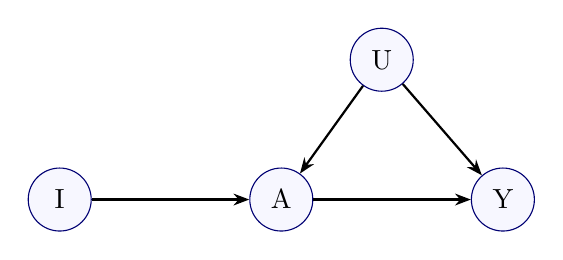
\begin{tikzpicture}[node distance=20mm]
\node[v] (i) {I};\node[v,right=of i] (a) {A};\node[v,right=of a] (y) {Y};\node[v,above right=12mm and 7mm of a] (u) {U};
\draw[edge] (i)--(a);\draw[edge] (a)--(y);\draw[edge] (u)--(a);\draw[edge] (u)--(y);
\end{tikzpicture}
\end{center}
The core linear IV assumptions are:
\begin{enumerate}
\item \textbf{Relevance:} $$\Cov(I,A)\neq0$$. The instrument shifts treatment.
\item \textbf{Exclusion:} the instrument affects the outcome only through treatment, so no direct effect or alternative directed route bypasses $$A$$.
\item \textbf{Exogeneity / independence:} the instrument is unrelated to the outcome disturbance containing unmeasured confounding. In the linear moment formulation, $$\Cov(I,\epsilon)=0$$; full nonparametric IV independence is stronger.
\end{enumerate}
Graphically, the combined exclusion and exogeneity requirements are often checked by d-separating $$I$$ and $$Y$$ after removing outgoing edges from $$A$$, written $$G_{\underline A}$$. This graph differs from the intervention graph $$G_{\overline A}$$, which removes \emph{incoming} edges.
\begin{correction}[Do not conflate exclusion with independence]
A direct path $$I\to Y$$ violates exclusion. A latent route linking $$I$$ to the outcome disturbance violates exogeneity. The d-separation statement in $$G_{\underline A}$$ incorporates both sorts of routes. In a linear SCM, correlation-based moment assumptions can be weaker than full probabilistic independence. Neither exclusion nor exogeneity is generally verifiable from the observed three-variable distribution alone.
\end{correction}

\section{Linear IV, the covariance ratio, and 2SLS}
\source{stat566-note5, p. 2; Lecture 8, Section 2}
Consider independent exogenous variables in
\begin{align}
I&\leftarrow\epsilon_I, & U&\leftarrow\epsilon_U,\\
A&\leftarrow\alpha_0+\alpha_1 I+\alpha_2 U+\epsilon_A,\\
Y&\leftarrow\beta_0+\beta_1 A+\beta_2 U+\epsilon_Y.
\end{align}
The homogeneous unit treatment effect (per unit change of continuous $$A$$, or a 0-to-1 contrast when appropriate) is $$\beta_1$$. Exogeneity and exclusion imply
\begin{align}
\Cov(I,A)&=\alpha_1\Var(I),\\
\Cov(I,Y)&=\beta_1\Cov(I,A)=\alpha_1\beta_1\Var(I),\\
\beta_1&=\frac{\Cov(I,Y)}{\Cov(I,A)}.
\end{align}
The sample covariance ratio is the just-identified IV estimator. With a binary instrument it equals the Wald ratio of differences in means:
\begin{equation}
\widehat\beta_{\mathrm{Wald}}=
\frac{\overline Y_{I=1}-\overline Y_{I=0}}
{\overline A_{I=1}-\overline A_{I=0}}.
\end{equation}
Indirect least squares divides the reduced-form slope from regressing $$Y$$ on $$I$$ by the first-stage slope from regressing $$A$$ on $$I$$.

Two-stage least squares (2SLS) generalizes to several instruments:
\begin{enumerate}
\item Regress $$A$$ on the instrument(s), with an intercept; obtain fitted values $$\widehat A$$.
\item Regress $$Y$$ on $$\widehat A$$, with an intercept; its slope is the 2SLS point estimate.
\end{enumerate}
\begin{remarkbox}[Inference needs the IV variance formula]
Ordinary second-stage OLS standard errors are incorrect because they treat the fitted treatment as the actual regressor in the error model. Use an IV implementation with suitable heteroskedasticity-robust or cluster-robust inference. The second-stage regression is not the reduced form; ``reduced form'' refers to $$Y$$ regressed on instruments and exogenous controls.
\end{remarkbox}
The open path $$A\leftarrow U\to Y$$ biases OLS on $$A$$. For $$I$$ and $$Y$$, however, $$I\to A\leftarrow U\to Y$$ has a collider at $$A$$ and is blocked without conditioning on $$A$$. This is why latent confounding need not contaminate the instrument's reduced-form variation.

\section{Conditional instruments and the Card example}
\source{stat566-note5, pp. 3--4; Lecture 8, Section 3}
With observed pre-treatment controls $$Z$$, valid instrument variation may be exogenous only after conditioning on $$Z$$. A constant-effect model is
\begin{equation}
Y=\beta A+g(Z)+\epsilon,\qquad \E[\epsilon\mid I,Z]=0,
\end{equation}
with relevant residual variation in $$I$$ predicting $$A$$. In the linear-controls case, include the same exogenous controls in both stages:
\begin{align}
A&\sim I+Z &&\text{first stage},\\
Y&\sim\widehat A+Z &&\text{second stage}.
\end{align}
Equivalently, residualize $$I,A,Y$$ on $$Z$$ and form the covariance ratio of residuals.
\begin{correction}[Controls belong in both stages]
The manuscript's second stage omits $$Z$$. Omitting it generally does not implement conditional IV. A ratio of conditional covariances at a particular $$z$$ can identify a constant effect under conditional moment assumptions, but it is not an instruction to divide arbitrary sample conditional covariance estimates or to average ratios without specifying weights.
\end{correction}
\begin{remarkbox}[Margin question: what if the proposed control is caused by the instrument?]
Whether conditioning on $$Z$$ is valid depends on its full causal role. A post-instrument mediator or collider can remove useful first-stage variation or induce selection bias. If $$I\to Z\to Y$$ bypasses $$A$$, unconditional exclusion fails. Treating $$Z$$ as an ordinary baseline control requires a new causal justification and overlap/relevance analysis, not merely adding it to both regressions. The small handwritten graph asks this question but does not establish a valid general rule.
\end{remarkbox}

The Card (1995) example uses proximity to college as an instrument for schooling and wages as the outcome. Family background and demographics can affect proximity, schooling, and wages. The instrument needs a credible argument that proximity has no remaining route to wages other than schooling after appropriate controls; local labor-market conditions illustrate a possible exclusion violation. The example motivates an identification strategy, not proof of instrument validity.

\section{Diagnostics, weak instruments, and exclusion sensitivity}
\source{stat566-note5, pp. 5--6; Lecture 8, Section 4}
A useful report distinguishes strength, validity assumptions, and the comparison to OLS.
\begin{enumerate}
\item \textbf{First-stage strength.} Report the excluded-instrument first-stage test and an appropriate robust version. The familiar $$F>10$$ is a rough heuristic, not a universal guarantee of reliable Wald inference. Weak instruments can make the covariance ratio unstable and invalidate usual normal approximations.
\item \textbf{Exclusion sensitivity.} Quantify how plausible direct instrument effects would change the result. This addresses an assumption that first-stage strength cannot test.
\item \textbf{OLS versus IV.} Durbin--Wu--Hausman tests assess disagreement under maintained instrument validity and model assumptions. Non-rejection does not prove no confounding or automatically justify choosing OLS; low power and weak instruments matter. A difference can also arise from invalid IVs or different heterogeneous-effect targets.
\end{enumerate}

Conley--Hansen--Rossi sensitivity analysis allows a direct effect $$\gamma$$:
\begin{equation}
Y=\beta A+\gamma I+Z^\top\delta+\epsilon.
\end{equation}
For each substantively plausible $$\gamma$$, run IV using $$Y-\gamma I$$ as the outcome. With residuals after removing $$Z$$,
\begin{equation}
\widehat\beta(\gamma)=
\frac{\widehat{\Cov}(\widetilde I,\widetilde Y)-
\gamma\widehat{\Var}(\widetilde I)}
{\widehat{\Cov}(\widetilde I,\widetilde A)}.
\end{equation}
Report the union of confidence intervals over the chosen range. The direct effect required to make the \emph{point estimate} zero differs from the magnitude at which a confidence interval first includes zero.

Anderson--Rubin inference tests a candidate $$\beta_0$$ by assessing whether the instrument predicts $$Y-\beta_0A$$ after controls. Inverting such tests produces confidence sets that can remain valid under weak identification with the corresponding error assumptions and test calibration; these sets may be wide or unbounded. Strong first-stage prediction does not protect against exclusion or exogeneity violations.
\begin{remarkbox}[Unexpanded remark, p. 6]
The manuscript includes ``DID for IV -- Ting Ye.'' This is retained as a reading prompt. Neither a complete estimator nor the required assumptions are specified there; it should not be interpreted as an established DiD-IV identification result in these notes.
\end{remarkbox}

\section{Partially linear IV and flexible nuisance fitting}
\source{stat566-note5, p. 7; Lecture 8, Section 5}
Keep a constant linear treatment effect but allow nonlinear covariate effects:
\begin{equation}
Y=\beta A+g(Z)+\epsilon,\qquad \E[\epsilon\mid I,Z]=0.
\end{equation}
Estimate the conditional means $$m_Y(z)=\E[Y\mid Z=z]$$, $$m_A(z)=\E[A\mid Z=z]$$, and $$m_I(z)=\E[I\mid Z=z]$$. Form
\begin{equation}
\widetilde Y=Y-\widehat m_Y(Z),\quad
\widetilde A=A-\widehat m_A(Z),\quad
\widetilde I=I-\widehat m_I(Z).
\end{equation}
The residualized moment suggests
\begin{equation}
\widehat\beta_{\mathrm{PLIV}}=
\frac{\sum_i\widetilde I_i\widetilde Y_i}
{\sum_i\widetilde I_i\widetilde A_i}.
\end{equation}
At the population nuisance functions,
\begin{equation}
\E[(I-m_I(Z))\{Y-m_Y(Z)-\beta(A-m_A(Z))\}]=0.
\end{equation}
Relevance requires a nonzero denominator. Cross-fit flexible nuisance estimates: train on other folds and predict each held-out fold. Cross-fitting limits overfitting bias but does not replace rate, moment, or relevance assumptions. The manuscript leaves the final coefficient blank; this ratio completes it under the stated model.

\section{Multiple instruments}
\source{stat566-note5, p. 8 heading; Lecture 8, Section 6 supplement}
With instrument vector $$I$$, project treatment onto all instruments and exogenous controls in the first stage. For a full instrument matrix $$Q$$ (including controls and intercept) and regressor matrix $$X$$,
\begin{equation}
\widehat\theta_{\mathrm{2SLS}}=(X^\top P_QX)^{-1}X^\top P_QY,
\qquad P_Q=Q(Q^\top Q)^{-1}Q^\top.
\end{equation}
This requires appropriate rank and full-column-rank conditions. More instruments do not automatically improve finite-sample performance, especially when many are weak.
\begin{supplement}[Overidentification tests have a qualified interpretation]
Sargan or robust Hansen--J tests assess the compatibility of extra instrument moments with a common structural parameter. Non-rejection does not prove all instruments valid. Under heterogeneous effects, distinct valid instruments can shift different complier populations and identify different LATEs; rejection may then reflect failure of the common-effect model rather than a simple exclusion violation.
\end{supplement}

\section{Binary IV and local average treatment effects}
\source{stat566-note5, p. 9 heading and p. 3 margin; Lecture 8, Section 7 supplement}
For binary instrument and treatment, let $$A(i)$$ denote treatment uptake under instrument value $$i$$. Under exclusion, write outcomes as $$Y(a)$$, independent of the instrument's direct value. The compliance types are
\begin{center}
\begin{tabular}{lcc}\toprule
Type & $$A(0)$$ & $$A(1)$$\\\midrule
Complier &0&1\\
Always-taker &1&1\\
Never-taker &0&0\\
Defier &1&0\\\bottomrule
\end{tabular}
\end{center}
Assume consistency, exclusion, instrument independence of the full potential-outcome and potential-treatment schedule, relevance, and monotonicity $$A(1)\geq A(0)$$ (no defiers). Then
\begin{align}
\E[A\mid I=1]-\E[A\mid I=0]&=\Prob(\text{complier}),\\
\E[Y\mid I=1]-\E[Y\mid I=0]
&=\Prob(\text{complier})\E[Y(1)-Y(0)\mid\text{complier}],\\
\frac{\E[Y\mid I=1]-\E[Y\mid I=0]}
{\E[A\mid I=1]-\E[A\mid I=0]}
&=\operatorname{LATE}.
\end{align}
Always-takers and never-takers do not change treatment when the instrument changes and contribute zero to the reduced-form contrast. Compliers do change treatment, and monotonicity rules out the opposite-sign contribution of defiers.
\begin{correction}[IV need not identify the population ATE]
The covariance ratio identifies $$\beta$$ in the constant-effect linear model. Under binary nonparametric assumptions it instead identifies LATE for compliers. It need not equal ATE or ATT. Different instruments may have different compliers and hence different causal targets. The response types based on $$Y(0),Y(1)$$ in Note 1 are distinct from these compliance types based on $$A(0),A(1)$$.
\end{correction}
Without monotonicity, a binary IV can still constrain the ATE through partial-identification bounds, but the simple LATE interpretation above no longer follows. This extends the Manski perspective: more structure can narrow an identified set without determining every population effect.

\section{Mendelian randomization}
\source{stat566-note5, p. 10; Lecture 8, Section 9}
Mendelian randomization uses genetic variants as instruments for an exposure. The graph in the manuscript connects a gene to disease/exposure and then to outcome, with demographics and other genes providing possible additional causes. Genetic allocation is not by itself proof of valid IV assumptions.
\begin{itemize}
\item Relevance: the variant predicts exposure.
\item Exogeneity: population stratification, relatedness, assortative mating, and other pathways must not confound the instrument--outcome relation.
\item Exclusion: horizontal pleiotropy (effects on outcome through routes other than exposure) can violate the assumption. Correlated variants also require attention to linkage disequilibrium.
\end{itemize}
In two-sample MR, instrument--exposure and instrument--outcome associations are estimated in separate samples for the same harmonized variants. For one variant the ratio is
\begin{equation}
\widehat\beta_{\mathrm{MR}}=\frac{\widehat\beta_{IY}}{\widehat\beta_{IA}}.
\end{equation}
Comparable populations, aligned effect alleles, and compatible association scales are required. Combining many variants needs assumptions and methods addressing dependence, weak instruments, and pleiotropy. The causal effect target also depends on the structural assumptions and the exposure variation induced by the instruments.
\section*{Lecture cross-reference}
Ema Perkovi\'c, STAT 566, Spring 2026: Lecture 8, \emph{Instrumental Variables}, Sections 1--7 and 9. The multiple-IV and binary-IV pages contain headings only; their text above is explicitly lecture-based supplementation. See \texttt{SOURCE-MAP.md} for coverage and unresolved annotations.

\end{document}
